
\begin{abstract}
A diabetes diagnosis entails important consequences for those receiving it. They receive important health information but also face the challenges of treating their disease. We investigated the causal effect of a diabetes diagnosis on health behaviours as well as on employment chances, two potentially intertwined factors. We used longitudinal data from the \ac{CHNS}, covering 1997 to 2011. Two complementary statistical techniques---marginal structural models and fixed effects---were used to estimate the causal effect a diabetes diagnosis on alcohol consumption, smoking, BMI, waist circumference and daily calorie consumption as well as employment probabilities. Both models suggested adverse associations with female employment chances (over 11 percentage points) and significant reductions in male \acf{BMI}, waist circumference and calorie consumption. These reductions were sustained over time. The effects on behavioural outcomes for women were smaller and less consistent. The Chinese healthcare system needs to particularly address the needs of women with diabetes as they experience the most severe consequences and are unlikely to achieve a change in health behaviours. Future research is needed to unravel the mechanism behind these sex differences.

\end{abstract}


\section{\label{sec:Introduction5}Introduction}

While the risk factors for type 2 diabetes, post diagnosis blood glucose management and the resulting complications of poor management have received much attention and are quite well researched---even in the context of China \parencite{Pan2015,Batis2014,Zhao2012,Ma2014,Chan2014,Yang2012}---, the impact of health information received at diabetes diagnosis on health behaviours and economic outcomes is less well known. This is despite research suggesting that behaviour changes after a diabetes diagnosis can have positive effects and reduce the risk of subsequent cardiovascular events\parencite{Long2014} and may help in effectively managing blood glucose levels and achieving further treatment goals \parencite{Zhou2016}.

Such information may be particularly important for \acp{LMIC} such as China, where diabetes prevalence has surged from 1\% in the early 1980s to about 10\% in recent years \autocite{Hu2011,Risk2016}. Confronting this diabetes epidemic puts a strain on healthcare systems \parencite{Seuring2015a}, increasing the need to find highly cost-effective prevention and treatment options in very resource constraint settings. However, to do this it is important to assess how successful the current system is in promoting positive health behaviours that are known to reduce the burden of diabetes.

So far, population-level research on the effects of health information on post-diagnosis behaviour change is scarce and has been limited to high-income countries. The sole study on the effects of recently diagnosed diabetes found positive behaviour changes shortly after diagnosis in a USA population. However, the effects were mostly short lived and tended to dissipate over time, particularly considering weight loss \autocite{Slade2012}. Slade created an "at risk" control group without diabetes that intended to be similar to the treatment group with diabetes, apart from not having received a diagnosis. He used information on diabetes biomarkers to estimate the propensity score of those without a diabetes diagnosis to be above a specific at risk threshold, so that everybody above a certain propensity score was used to form the control group. He then estimates dynamic population averaged as well as \ac{FE} models for identification. While this allowed for the construction of a potentially better control group, the study was not able to account for the possibility of selection into treatment based on pre-treatment values of the dependent variables.

Another study investigated the effect of a hypertension diagnosis on nutritional behaviours in China using a quasi-experimental regression-discontinuity design and biomarker information on blood pressure \autocite{Zhao2013a}. It was assumed that people above the hypertension threshold were informed about that result while those just below the threshold were not. These two groups were then compared to isolate the particular effect of the additional health information on food consumption. The results indicated that a diagnosis leads to reductions in fat consumption of the rich, at the consecutive wave 3--4 years later. However, an important caveat of the study is the assumption that everybody above the threshold was informed and everybody below the threshold did not receive this information. This is a strong assumption as it was unclear if the participants received just the actual blood pressure measurement information and had to interpret these data themselves, or if they were made aware of their hypertension or also pre-hypertensive status \autocite{Zhao2013a}. Further, the results are only applicable to the population around the hypertension threshold, while effects might be different for people receiving this information and having very severe hypertension already.

%Finally, another study on China also used diabetes biomarkers to identify those formally unaware of their diabetes, assuming that they were informed about their diabetes status by the survey team \parencite{Liu2014}. They use a difference in difference approach to identify the effect of a diagnosis on labour income in the wave after diagnosis, finding a decrease of about 16\%. They attribute this effect to the psychological consequences of the diabetes diagnosis, however, they are not able to rule out an effect of a deterioration of health on income. Further, the results only provide a short term picture, and it remains unclear if people are able to recover from the initial shock. ONLY INCLUDE IF I ALSO LOOK AT INCOME

This study contributes in several ways to the existing literature. First, it provides information on the effect of a diabetes diagnosis on health behaviours and employment in China, not only over the short term, but for a period covering the entire decade of the 2000s, allowing for a more long term investigation of the effects. Second, it deals with the challenge of selection into diagnosis in two ways, accounting for both selection due to unobserved time-invariant and observed time-variant confounders using a \ac{FE} approach. For example, specific characteristics such as motivation, could affect the propensity to visit a doctor and receive a diagnosis as well as to engage in health behaviour changes or to be employed, potentially leading to biased estimates if unaccounted for. Further, it also accounts for selection into diagnosis due to observed time-variant factors, such as pre-diagnosis changes in our outcomes of interest, using \acp{MSM}. Again, if such predetermination existed results would be biased, preventing a causal interpretation.  

We used panel data from six waves of the \acf{CHNS}, spanning the period from 1997 to 2011. The survey provides one of the most comprehensive sources of data on nutrition and health in China and has been used widely in epidemiological and economic studies, particularly to investigate the causes of nutrition and health changes over the last two decades \parencite{Zhang2014d}. We hypothesized that a diagnosis of diabetes leads to positive behaviour change, at least initially after diagnosis, but at the same time reduces employment probabilities. We investigated both, the overall average change in outcomes after a diagnosis as well as the time trends. 
\section{\label{sec:Methods5}Methods}

\subsection{Study sample}

The \ac{CHNS} is an international collaborative project led by the Carolina Population Center at the University of North Carolina at Chapel Hill investigating nutrition and health behaviours in nine provinces of China \parencite{Zhang2014d}. We use data from 1997 onwards, which was the first time survey participants provided diabetes information. In total we use six waves (1997, 2000, 2004, 2006, 2009 and 2011) obtained from the longitudinal dataset released in 2015. The data provide extensive information on nutrition and health, including anthropometric measures of weight and height, reducing potential measurement issues. It further provides socioeconomic information, most importantly for this study about employment. The sample is limited to the adult population from age 18--64.  The sample is not nationally representative and as such does not provide sampling weights  \parencite{Popkin2010}.

Overall, between 84\% to 90\% are followed up in the following wave, with attrition being highest after 2006. Attrition in the \ac{CHNS} due to mortality is around 1\%in the \ac{CHNS} \parencite{Popkin2010}. Other reasons mentioned by \textcite{Popkin2010} are loss to follow up due to migration and natural disasters and redevelopment of housing in the urban centres leading to relocations. We analysed if any of our variables of interest was significantly related to attrition and did only find lower calorie consumption to be predict attrition. Further, attrition was related to urbanization, higher education and being of younger age, suggesting that mostly younger, more urbanized participants tended to leave the survey. Given the generally older population of people with diabetes we are interested in, we do not think that attrition will affect our estimates to any major extend. IS THIS SUFFICIENT REGARDING ATTRITION OR SHOULD I DO ANY FURTHER ANALYSIS. SO FAR I ONLY REGRESSED ATTRITION ON THE VARIABLES WE USE IN THIS PAPER.


\subsection{Assessment of diabetes}

We used self-reported information on a diabetes diagnosis to construct our diabetes indicator. We only relied on incident cases of self-reported diabetes, excluding individuals with self-reported diabetes at baseline. Given the chronic nature of diabetes, we assumed that after the initial diagnosis diabetes persisted for the rest of one's life. To construct a measure of diabetes duration for incidence cases we used self-reported information on the year of diagnosis. If we found that the year of diagnosis was reported to be before the last wave without a reported diagnosis, we used the midpoint between the last wave without diagnosis and the first wave with a diagnosis as the year of diagnosis. 

\subsection{Assessment of outcomes}

The behavioural outcomes we estimated were current smoking status, any alcohol consumption over the last year, \ac{BMI}, waist circumference in centimetres and daily calorie consumption. Smoking status and alcohol consumption were self-reported, while \ac{BMI} and waist circumference were based on anthropometric measures, minimizing potential reporting errors. Waist circumference is reported in centimetres. Finally, daily calorie consumption is a constructed variable available in the \ac{CHNS}, based on the average daily consumption of carbohydrates, protein and fat of every individual in the survey, measured on three consecutive days. Our economic outcomes was employment status, based on a self-reported measure of if the person was currently working. People who were not working because they were students were excluded. We did include those that were not working due to any other reason such as doing housework, being disabled or being retired.


\subsection{Statistical analysis}


We used two statistical approaches to account for potential confounding: \acfp{MSM} and \acf{FE}. 

\subsubsection*{Marginal structural models}

\acp{MSM} apply inverse probability weights to adjust for confounding and selection bias as a result of time-varying confounders being affected by prior exposure \autocite{Robins2000}. Under the assumption of the \ac{MSM}\autocite{Robins2000}---the reported treatment is the treatment that has actually been received (consistency), there are no unmeasured confounders (exchangeability) and every person in the sample has a non-zero chance of receiving the treatment (positivity) (see Section \ref{sec:Discussion5} for a discussion of the validity of these assumptions in our case)---the causal DAG shown in Figure \ref{fig:DAG} displays the association between confounders and outcomes and a diabetes diagnosis. This causal graph was drawn using DAGitty program version 2.3.\autocite{Textor2011}.

\begin{figure}
\begin{center}
\caption{\label{fig:DAG} Direct acyclic graph (DAG) representing the relations between confounders/outcomes and a diabetes diagnosis.}
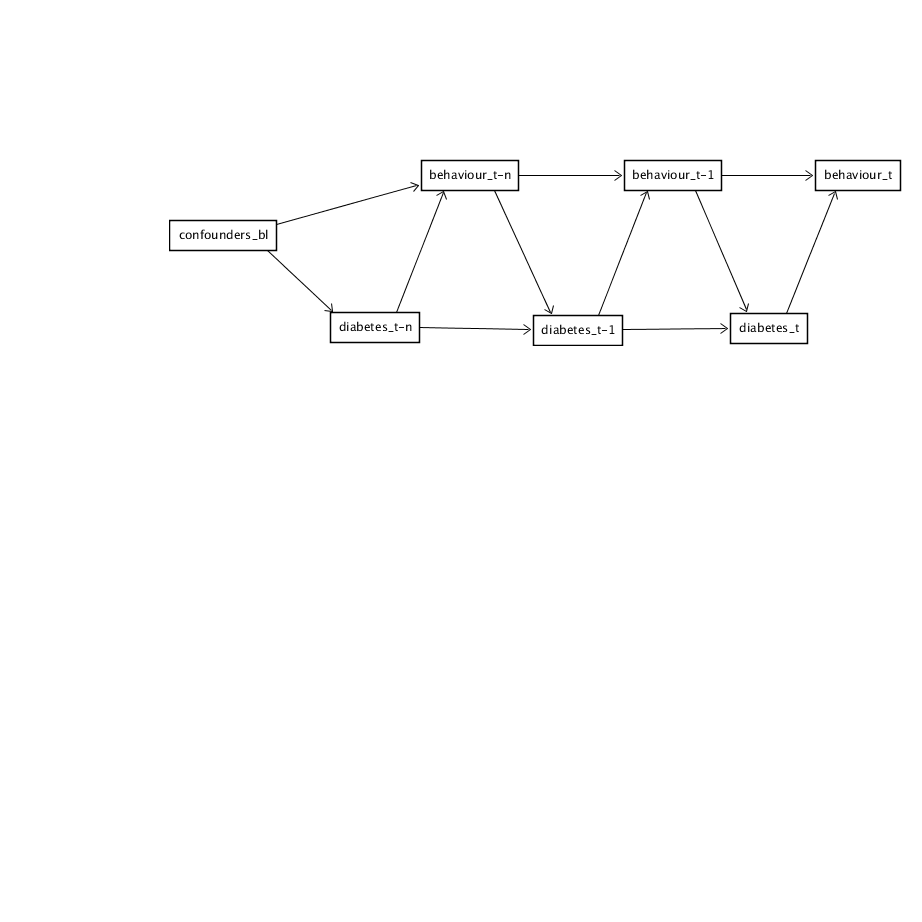
\includegraphics[scale=0.7]{Chapter5/Figures/dag}
\end{center}
\footnotesize{\textit{Notes} The confounders not only include control variables but also pre-treatment values of our outcomes of interest to account for any predetermination of the treatment.}

\end{figure}


We accounted for two sets of confounders: time-varying variables at baseline as well as lagged time-varying variables in the waves following the baseline, to capture the effects of changes in these variables over time. In our context it seemed possible that, for example, \ac{BMI} could affect the probability of being diagnosed with diabetes which then itself may affected subsequent \ac{BMI} levels, confounding the relationship between a diabetes diagnosis and \ac{BMI} due to non-random selection. Similarly  employment history and current employment could affect the probability of self-reporting a diabetes diagnosis through their impact on lifestyle, potentially due to an increase in disposable income or a reduction in leisure time, potentially confounding the relationship between a diabetes diagnosis and employment status. We used time-invariant variables lagged by one period to prevent reverse causality in the prediction of diabetes risk. Because current diabetes status as reported in the survey was determined at some point within the current and the previous wave, we had to use confounders from the previous wave determined before the current diabetes status, to prevent reverse causality.

Using \ac{MSM} and creating inverse probability of treatment weights, we were able to construct a pseudo population, based on the person's potential exposure at each time point, that allowed us to adjust the estimates for confounding due to selection. We first constructed unstabilized weights using baseline values of the time-invariant and time-variant confounders as well as time-variant confounders lagged by one period to predict the probability of developing diabetes at each wave. The used predictors were age and age squared to account for changes in risk with increasing age, an index of urbanization pre-constructed within the \ac{CHNS} data, ranging from 1 to 120 as the level of urbanization increases \parencite{Zhang2014d}, to account for the impact of urbanization on diabetes risk \parencite{Attard2012}. We also used secondary and university education, being married, having any medical insurance, being of Han ethnicity, living in a rural area, dummies for the different Chinese regions and the respective survey waves as predictors. Further we used inflation adjusted per-capita household expenditures to predict any effects of household wealth on diabetes. Finally, all outcome variables (employment status, alcohol consumption, smoking status, \ac{BMI}, waist circumference and average daily calorie consumption) were used as predictors. 

Because unstabilized weights can be highly variable it is recommended to stabilize the weights \parencite{Cole2008}. Using the unstabilized weights as the denominator, stabilized weights were calculated by dividing the denominator by the predicted treatment propensity from a model using only time-invariant confounders and baseline information of the time-variant confounders as predictors.  Because our analysis was stratified by males and females, we created weights separately for both groups.

The \acp{MSM} were estimated using \ac{OLS} for the continuous and a logistic model for the binary outcomes. For the logistic model we calculated marginal effects and present them instead of odds ratios for greater comparability with the results of the \ac{FE} models. All models were weighted by the stabilized weights constructed beforehand while adjusting for all baseline and time-invariant covariates used in the calculation of the stabilized weights, except for the respective outcome of interest. Robust standard errors to account for intra-class correlation of repeated outcome measurements in individuals were used throughout. In our primary analysis, we present the results of the \ac{MSM} with untruncated stabilized weights, as these present unbiased estimates, albeit they likely are less efficient than truncated weights \parencite{Cole2008}.

\subsubsection*{Fixed effects}

While the \ac{MSM} can account for pre-treatment selection on observable and time-variant confounders, it assumes that there are no time-invariant unobserved confounders such as family background, cognitive abilities, motivation and other personal characteristics. This is a strong assumption that may be violated. The individual level \ac{FE} model can help remedy this problem as it is able to account for both observed time-variant variables and time-invariant unobserved variables. It does so by demeaning the confounding variables by the mean of the confounder over all observed time points for an individual. It then uses solely the within-person variation for identification, thereby accounting for any time-invariant observed or unobserved as well as observed time-variant effects. 

 Due to the demeaning, time-invariant variables such as Han ethnicity, were dropped from the model and could not be estimated. Further, because the \ac{FE} model is not able to account for any treatment effects on other time-variant confounders, only a more limited set of confounders could be included compared to the \ac{MSM}. Otherwise our estimate of the effect of a diabetes diagnosis would likely be biased due to the inclusion of bad controls \parencite{Angrist2009a}. Bad controls are controls that have been affected by the treatment itself---such as \ac{BMI} or smoking status after a diabetes diagnosis---and therefore likely capture part of the causal effect of diabetes on our outcome of interest, biasing the diabetes coefficient \parencite{Angrist2009a}. The \ac{FE} models thus only included controls for age, age squared, the level of urbanization, education, being married, having any medical insurance, living in a rural area, and dummies for the different Chinese regions and the respective survey waves. For the estimation of the effect of time since diagnosis, the linear age variable was dropped. In \ac{FE} models, two or more variables that change at the same rate between waves cannot be separately identified. Here this was the case with age and time-dummies, as both variables increased by one each additional year \parencite{Wooldridge2012}. To identify the effect of diabetes duration we had to rely on the presence of people without diabetes in the sample, for which diabetes duration did not increase at the same rate as time.

Because it is not possible to retrieve marginal effects from a logistic \ac{FE} model, we used a \ac{FE} linear probability model instead. It generally produces very similar estimates compared to non-linear models \parencite{Angrist2009a}. COMMENT TILL: CAN ALSO ADDITIONALLY PRESENT RESULTS FROM LOGIT MODELS IF NEEDED TO SHOW THAT THEY INDICATE SIMILAR EFFECTS. NOT SURE IF NEEDED AS THIS MEANS A LOT MORE TABLES

\subsubsection*{Multiple imputation}

To deal with missing data, we used chained multiple imputation to impute the missing values in Stata 13 using the user written ICE command \parencite{Royston2009}. Imputation models included all variables used in the \acp{MSM}. We did not impute missing diabetes information and instead assumed that once a diabetes diagnosis was reported, the individual had diabetes in every ensuing wave, even when the observation was missing. If diabetes was never reported in any wave, we assumed that the individual never had diabetes. Consequently, we only imputed missing values for those observations that had a non-missing diabetes status. For the calculation of the marginal effects in the \ac{MSM} logit models, Rubin's rules were applied using the user written Stata command mimrgns \parencite{Klein2014}.

\subsubsection*{Number of observations}

Because we used lagged variables to construct the stabilized weights for the \acp{MSM}, the number of observations used in the \acp{MSM} was lower than those used in the \ac{FE} models, where we did not use lagged variables. The summary statistics shown in Table \ref{tab:descriptives_diab} are based on the observations used in the \ac{FE} models.

\subsubsection*{Sensitivity analyses}

We conducted three additional sensitivity analyses in order to test the robustness of our results to different assumptions and estimation strategies.
First, we truncated weights at the 1\textsuperscript{st} and 99\textsuperscript{th} percentile to investigate the sensitivity of the \acp{MSM} to the most extreme weights. While untruncated weights provide unbiased estimates under the assumptions of the \ac{MSM}, they may not be the most efficient and tend to have larger standard errors \parencite{Cole2008}. Second, we estimated all models using only covariate adjustment to investigate in how far this 'naive' approach diverts from the "causal" estimates of the \ac{FE} and \acp{MSM}. Third, we estimated the \ac{FE} and \acp{MSM} using the original non-imputed data to ascertain the extend to which multiple imputation affected the results.

\section{\label{sec:Results5}Results}

From the descriptive statistics, we can observe that people with self-reported diabetes were less likely to be employed. Looking at health behaviours, it were mainly men that smoked and reported alcohol consumption while very few women did so. The prevalence of smoking and drinking was lower for men with diabetes; they also consumed fewer calories compared to men without diabetes. Further, the self-reported diabetes group had both higher \ac{BMI} and waist circumference levels. They were also older, lived in more urbanized areas, were more likely to have insurance and men were somewhat better educated while women were less educated compared to their counterparts without diabetes. Both men and women reported an average time since diagnosis of around 4 years. Interestingly, while there is no significant difference in household expenditures for men, women with diabetes come from families with significantly lower household expenditures, suggesting that they life in lower resource settings than women without diabetes. Overall it appears that in China it is less educated and poorer women that self-report a diagnosis, while self-reporting men are better educated and tend not to be poorer than their counterparts without diabetes.


\begin{landscape}
\begin{table}[h]
\caption{\label{tab:descriptives_diab}Sample means for males and females, by diabetes status}
\begin{center}
\begin{adjustbox}{max width=\linewidth}  
{
\def\sym#1{\ifmmode^{#1}\else\(^{#1}\)\fi}
\begin{tabular}{l*{6}{SS}}
\toprule
                    &\multicolumn{3}{c}{Males}             &\multicolumn{3}{c}{Females}           \\\cmidrule(lr){2-4}\cmidrule(lr){5-7}
                    &\multicolumn{1}{c}{No diabetes}&\multicolumn{1}{c}{Diabetes}&\multicolumn{1}{c}{p-value (t-test)}&\multicolumn{1}{c}{No diabetes}&\multicolumn{1}{c}{Diabetes}&\multicolumn{1}{c}{p-value (t-test)}\\
\midrule
Employed            &        81\%&        69\%&    0.000        &        66\%&        28\%&     0.000       \\
Smokes              &        59\%&        46\%&      0.000      &        3\%&        4\%&    0.000        \\
Any alcohol consumption&     64\%&        53\%&       0.000     &        9\%&        4\%&   0.000         \\
Daily Kcal eaten (3-day average)&     2438&     2149&      0.000      &     2065&     1919&   0.001         \\
BMI                 &       23.04&      25.22&       0.000     &       23.15&       25.89&    0.000        \\
Waist circ. (cm)    &       82.28&       89.70&      0.000      &       78.92&       88.04&     0.000       \\
Age                 &       43.33&      52.90&      0.000      &       43.70&       55.56&     0.000       \\
Han ethnicity       &        87\%&      89\%&     0.443       &        87\%&        91\%&     0.079      \\
Rural area          &        68\%&       51\%&     0.000       &        68\%&        48\%&     0.000       \\
Married             &        84\%&      95\%&     0.000       &        88\%&        85\%&    0.108        \\
Secondary education     &        64\%&      67\%&   0.401         &        49\%&        40\%&       0.006     \\
University education    &        6\%&      14\%&    0.000        &        4\%&        1\%&     0.017      \\
Any health insurance&        52\%&     82\%&     0.000       &        50\%&        67\%&       0.000      \\
Urbanization Index  &       61.27&     75.62&     0.000       &       61.92&       69.25&     0.000       \\
Household expenditures (Yuan (2011))&     5013.40&     4178.76&    0.927        &     4610.57&     1829.39&    0.020        \\
Years since diabetes diagnosis&       -&        3.93&      -      &        -&        4.22&      -      \\
\midrule
Observations        &       23413&         284&       23697&       23577&         336&       23913     \\
\bottomrule
\end{tabular}
}
\end{adjustbox}
\end{center}
\end{table}
\end{landscape}
\FloatBarrier

Predicting the denominator for the stabilized weights we find that for men a higher baseline \ac{BMI}, increasing age and increasing household expenditures have some predictive value for a diabetes diagnosis (Table \ref{tab:predictors}). For women, higher age at baseline, increases in \ac{BMI} and waist circumference  as well as living in a non-rural environment predict a diabetes diagnosis. Further, especially living in certain provinces of the country appears to increase the likelihood to receive a diabetes diagnosis for men, but not for women.

\begin{table}[h]
\caption{\label{tab:predictors}Time variant and invariant predictors of diabetes self-report (denominator of stabilized weights)}
\begin{center}
\begin{adjustbox}{max width=\linewidth}  
{
\def\sym#1{\ifmmode^{#1}\else\(^{#1}\)\fi}
\begin{tabular}{l*{4}{S S}}
\toprule
                &\multicolumn{2}{c}{Males}&\multicolumn{2}{c}{Females}\\\cmidrule(lr){2-3}\cmidrule(lr){4-5}&\multicolumn{1}{c}{(1)}&\multicolumn{1}{c}{(2)}&\multicolumn{1}{c}{(3)}&\multicolumn{1}{c}{(4)}\\
                &\multicolumn{1}{c}{$\beta$}&\multicolumn{1}{c}{SE}&\multicolumn{1}{c}{$\beta$}&\multicolumn{1}{c}{SE}\\
\midrule
Age (bl)          &-.001 &.001         &.004\sym{**} & .002         \\
Age squared (bl)       &.000 &.000         &-.000\sym{*} &.000         \\
Urbanization index (bl)      &.000 &.000         &-.000 & .000         \\
\ac{BMI} (bl)        &.001\sym{**} &.001         &.001 &.001         \\
Waist circumference (cm) (bl)        &.000 &.000         &.000 &.000         \\
3-Day Ave: Energy (kcal) (bl)       &-.000 &.000         &-.000 &.000         \\
Smoking (bl)    &.001 &.002         &.002 &.007         \\
Any alcohol (bl)        &.000 &.002         &.000 &.003         \\
Secondary educ. (bl)    &-.002 &.004         &.002 &.004         \\
University educ. (bl) &-.005 &.007         & -         \\
Married (bl)      &-.003 &.004         &-.000 &.005         \\
Any medical insurance (bl)    &.002 &.002         &-.001 &.002         \\
Employed (bl)        &.002 &.003         &.002 &.002         \\
Han ethnicity   &.002 &.003         &-.003 &.004         \\
Rural      &-.001 &.002         &-.005\sym{***} &.002         \\
Household expenditures (2011 Yuan) (bl)&-.000 &.000         &.000 &.000         \\
Survey year && \\
\hspace*{10mm}2004&.003 &.003         &-.003 &.003         \\
\hspace*{10mm}2006&.001 &.003         &-.004 &.003         \\
\hspace*{10mm}2009&.011\sym{***} &.004         &-.001 &.004         \\
\hspace*{10mm}2011&.001 &.003         &.001 &.004         \\
Age           &.004\sym{**} &.002         &-.002 &.002         \\
Age squared        &-.000\sym{***} &.000         &.000 &.000         \\
BMI          &-.001 &.001         &.001\sym{*} &.001         \\
Urbanization index         &.000 &.000         &.000 &.000         \\
Waist circumference (cm)         &.000\sym{*} &.000         &-.000 &.000         \\
3-Day Ave: Energy (kcal)        &-.000 &.000         &.000 &.000         \\
Smoking         &-.004\sym{*} &.002         &-.001 &007         \\
Any alcohol        &-.003 &.002         &-.006 &.004         \\
Secondary education     &.003 &.004         &.000 &.004         \\
University education    &.003 &.007         & -         \\
Married       &.000 &.005         &-.002 &.004         \\
Any medical insurance     &.002 &.002         &-.000 &.002         \\
Employed         &-.004\sym{*} &.002         &-.003 &.002         \\
Household expenditures (2011 Yuan) &.000\sym{**} &.000         &-.000 &.000         \\
\bottomrule
\multicolumn{5}{l}{\footnotesize \sym{*} \(p<0.10\), \sym{**} \(p<0.05\), \sym{***} \(p<0.01\)}\\
\multicolumn{5}{l}{\footnotesize Results for province dummies omitted to preserve space.}\\
\end{tabular}
}
\end{adjustbox}
\end{center}
\end{table}

The results of our regression analysis are presented in Table \ref{tab:binary}. Both the \ac{FE} model and the \ac{MSM} indicate that women self-reporting a diabetes diagnosis have reduced probabilities of being employed than their counterparts without diabetes, with a reduction of 11 percentage points in the \ac{FE} model and 12 percentage points in the \ac{MSM}. This translates into a relative reduction in employment probabilities between 16--17\%. For men no such effect is observed.

\begin{table}[h]

\caption{\label{tab:binary}Analysis of the effect of a diabetes diagnosis on employment status and behavioural outcomes using fixed effects and marginal structural models}
\begin{adjustbox}{max width=\linewidth, center}
\begin{threeparttable}  %adds notes to tables
{
\def\sym#1{\ifmmode^{#1}\else\(^{#1}\)\fi}
\begin{tabular}{l*{6}{S
S}}
\toprule
                &\multicolumn{1}{c}{(1)}&\multicolumn{1}{c}{(2)}&\multicolumn{1}{c}{(3)}&\multicolumn{1}{c}{(4)}&\multicolumn{1}{c}{(5)}&\multicolumn{1}{c}{(6)}\\
                &\multicolumn{1}{c}{Employment}&\multicolumn{1}{c}{Smoking}&\multicolumn{1}{c}{Any alcohol}&\multicolumn{1}{c}{BMI}&\multicolumn{1}{c}{Waist (cm)}&\multicolumn{1}{c}{Calories (kcal)}\\
                \midrule
&\multicolumn{6}{c}{\emph{Fixed effects}} \\  
\addlinespace                                   

Male sample &&&&&&\\
Diabetes&      .018         &    -.026         &    -.087\sym{***}&    -.727\sym{***}&   -2.215\sym{***}& -171.754\sym{***}\\
                &   (.030)         &   (.032)         &   (.034)         &   (.187)         &   (.590)         & (65.287)         \\
Female sample &&&&&&\\
Diabetes     &      -.110\sym{***}&    -.027\sym{**} &    -.023         &    -.668\sym{**} &   -1.177\sym{*}  &  -62.971         \\
                &   (.035)         &   (.013)         &   (.018)         &   (.264)         &   (.622)         & (55.960)         \\    
\midrule      
\addlinespace 
&\multicolumn{6}{c}{\emph{Marginal structural model}} \\
\addlinespace             
Male sample &&&&&&\\
Diabetes        & -.008         &    -.054\sym{*}  &    -.132\sym{***}&    -.785\sym{***}&   -1.686\sym{***}& -125.161\sym{*}  \\
                &   (.027)         &   (.030)         &   (.034)         &   (.188)         &   (.591)         & (66.311)         \\
Female sample &&&&&&\\
Diabetes        &   -.122\sym{***}&    -.017\sym{*}  &    -.076\sym{***}&    -.458\sym{*}  &    -.559         &  -60.878\sym{*}  \\
                &   (.030)         &   (.009)         &   (.023)         &   (.251)         &   (.633)         & (34.744)         \\                
\bottomrule
\end{tabular}
\begin{tablenotes}
\item \textit{Notes} Standard errors in parentheses. Other control variables: age (only MSM), age squared, region, urban, education, han, marital status, urbanization index, time dummies, health insurance status, household expenditures.  Fixed effects: N=23697 (male sample), N=23913 (female sample); MSM:  N=13231 (male sample), N=14630 (female sample).
\item \sym{*} \(p<0.10\), \sym{**} \(p<0.05\), \sym{***} \(p<0.01\))
\end{tablenotes}
}
\end{threeparttable}
\end{adjustbox}

\end{table}

There is a more ambiguous picture for the effect of a diabetes diagnosis on behavioural outcomes. There is no strong evidence that men reduced their smoking rate, however, a diabetes diagnosis likely led to a reduction in alcohol consumption as is shown by both models, but in particular the \ac{MSM}. For waist circumference, \ac{BMI} and calorie consumption, the \ac{FE} and \ac{MSM} both indicate reductions in \ac{BMI} of close to 0.7, of about 2 cm in waist circumference and of up to 170 calories per day for men. For women no similar evidence is found and while the point estimates indicate a reduction in all outcomes, these tend to be smaller than those for men and only statistically significant in the \ac{FE} model for \ac{BMI} and waist circumference.

Exploring the effect of a diabetes diagnosis over time, we first estimated a specification using time since diagnosis as a continuous variable. The results of the \ac{FE} model (Table \ref{tab:duration}) indicate a steady reduction of female employment probabilities of almost two percentage points per year and of male alcohol consumption, \ac{BMI}, waist circumference and consumed calories. The \ac{MSM} again supports the finding of the \ac{FE} model, finding very similar effects in terms of size and statistical significance. For women, the \ac{MSM} also support the finding of a reduction in employment probabilities, with the point estimate  being somewhat larger compared to the \ac{FE} model. The evidence for changes in health behaviours is less consistent across models and outcomes, with the \ac{FE} indicating a reduction in waist circumference but not in \ac{BMI} and the \ac{MSM} suggesting the opposite. The effect sizes for changes in health behaviours in women are about half the size to those found in men. 

\begin{table}[h]
\caption{\label{tab:duration}Analysis of the effect of time since diabetes diagnosis on employment status and behavioural outcomes using fixed effects and marginal structural models}
\begin{adjustbox}{max width=\linewidth} 
\begin{threeparttable}  %adds notes to tables
{
\def\sym#1{\ifmmode^{#1}\else\(^{#1}\)\fi}
\begin{tabular}{l*{6}{S S}} \toprule
                &\multicolumn{3}{c}{Odds ratios}                   &\multicolumn{3}{c}{Beta coefficients}         \\\cmidrule(lr){2-4}\cmidrule(lr){5-7}
                &\multicolumn{1}{c}{(1)}&\multicolumn{1}{c}{(2)}&\multicolumn{1}{c}{(3)}&\multicolumn{1}{c}{(4)}&\multicolumn{1}{c}{(5)}&\multicolumn{1}{c}{(6)}\\
                &\multicolumn{1}{c}{Employment}&\multicolumn{1}{c}{Smoking}&\multicolumn{1}{c}{Any alcohol}&\multicolumn{1}{c}{\ac{BMI}}&\multicolumn{1}{c}{Waist (cm)}&\multicolumn{1}{c}{Calories (kcal)}\\
                \midrule
&\multicolumn{6}{c}{\emph{Fixed effects}} \\
\addlinespace                     
Male sample &&&&&&\\
Time since diagnosis&   -.000         &    -.004         &    -.014\sym{**} &    -.155\sym{***}&    -.542\sym{***}&  -25.595\sym{**} \\
                &   (.008)         &   (.007)         &   (.007)         &   (.036)         &   (.111)         & (10.297)         \\
Female sample &&&&&&\\
Time since diagnosis&   -.018\sym{**} &    -.005\sym{**} &    -.002         &    -.087         &    -.260\sym{**} &  -11.696         \\
                &   (.007)         &   (.002)         &   (.003)         &   (.053)         &   (.122)         &  (8.946)         \\ 
\addlinespace 
\midrule
&\multicolumn{6}{c}{\emph{Marginal structural model}} \\               
\addlinespace
Male sample &&&&&&\\
Time since diagnosis   &  -.006         &    -.011\sym{*}  &    -.021\sym{***}&    -.151\sym{***}&    -.417\sym{***}&  -28.974\sym{***}\\
                &   (.005)         &   (.006)         &   (.006)         &   (.037)         &   (.103)         & (10.199)         \\
Female sample &&&&&&\\
Time since diagnosis  & -.025\sym{***}&    -.003\sym{*}  &    -.015\sym{***}&    -.117\sym{**} &    -.166         &  -10.991\sym{*}  \\
                &   (.006)         &   (.001)         &   (.006)         &   (.047)         &   (.124)         &  (6.338)         \\                 
\bottomrule
\end{tabular}
\begin{tablenotes}
\item \textit{Notes} Standard errors in parentheses. Other control variables: age (only MSM), age squared, region, urban, education, han, marital status, urbanization index, time dummies, health insurance status, household expenditures. Fixed effects: N=23697 (male sample), N=23913 (female sample); MSM:  N=13231 (male sample), N=14630 (female sample).
\item \sym{*} \(p<0.10\), \sym{**} \(p<0.05\), \sym{***} \(p<0.01\))
\end{tablenotes}
}
\end{threeparttable}
\end{adjustbox}
\end{table}

\FloatBarrier

In a second step we estimated a specification using year dummies to capture the potential non-linearity in the relationship between time since diagnosis and our outcomes. The results for both estimation methods are visualized in Figure \ref{fig:duration_g_fe_mi} and presented in Tables \ref{tab:duration_groups_fe} and \ref{tab:duration_groups_msm} for the \ac{FE} and \ac{MSM}, respectively. Despite the smaller sample size in each group and hence lower precision, the \ac{FE} model still indicates a reduction in \ac{BMI} and waist circumference for men, especially in the first 8 to 10 years after diagnosis. A similar effect is found for females, especially for years 3 to 8 after diagnosis. Interestingly, female employment already decrease rapidly in the 1 to 2 year after diagnosis and it does not appear that females are able to increase their chances later on. Using the \ac{MSM}, all point estimates suggest similar effects, but due to the lower sample size, we were not able to estimate the effects for females on smoking and alcohol consumption.


\begin{figure}
\begin{center}
\caption{\label{fig:duration_g_fe_mi} Analysis of the effect of time since diabetes diagnosis on employment status and behavioural outcomes using fixed effects and marginal structural models (duration groups)}

Fixed effects
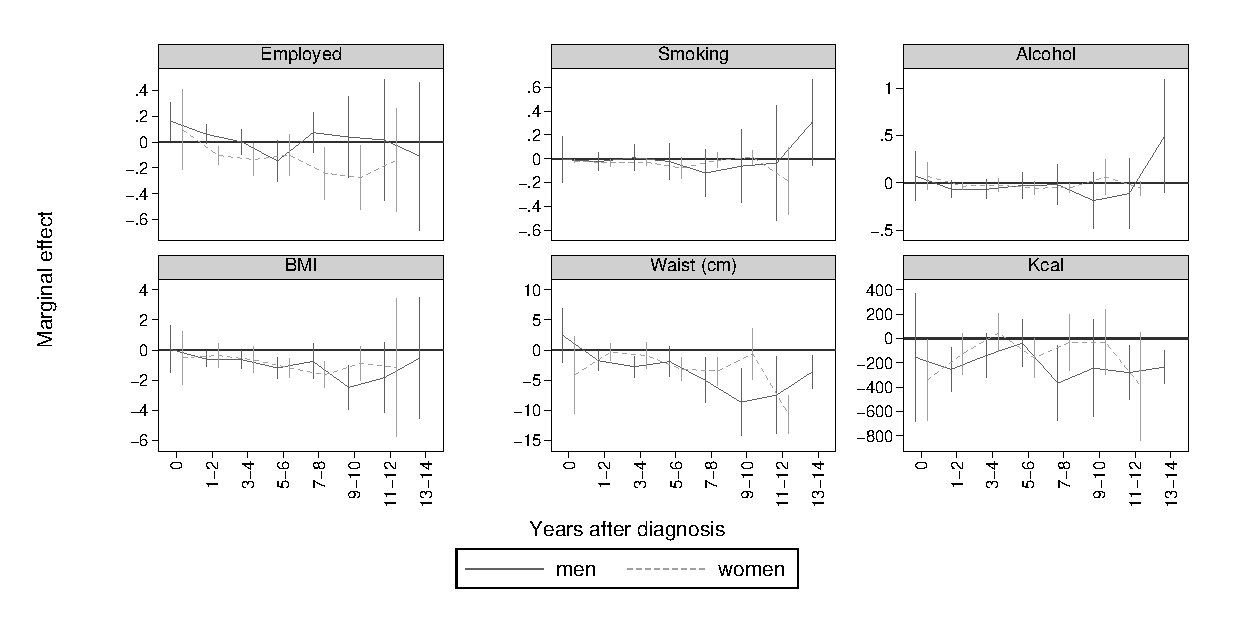
\includegraphics[width=\linewidth]{Chapter5/Figures/mi_fe}
Marginal structural models
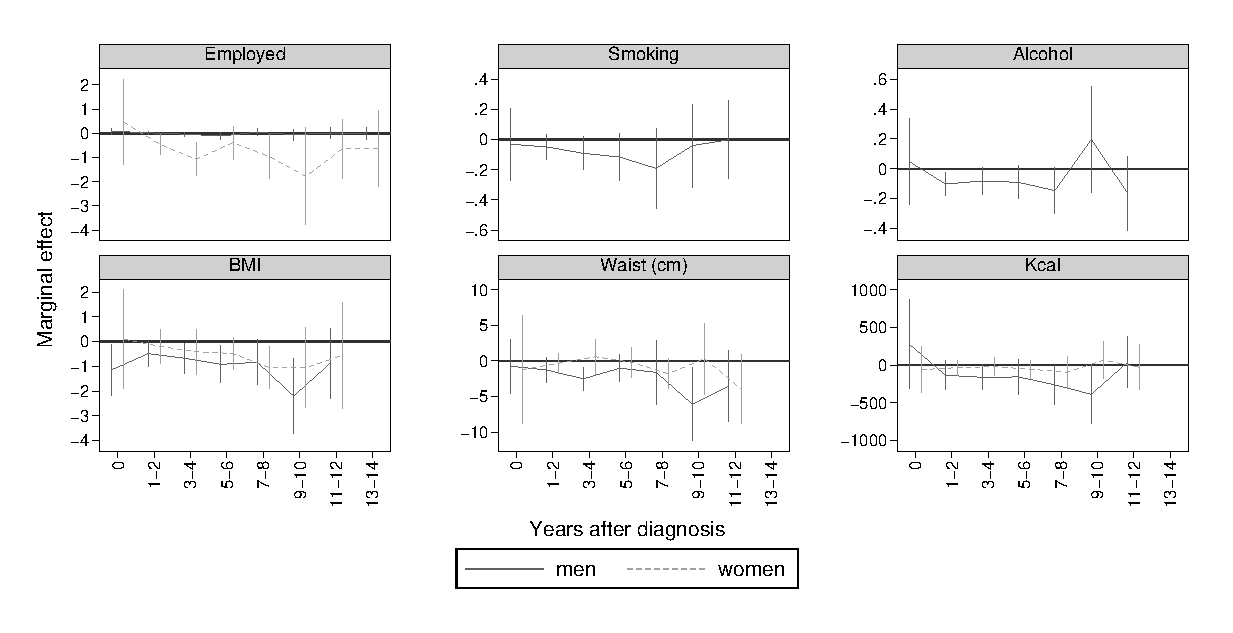
\includegraphics[width=\linewidth]{Chapter5/Figures/mi_msm_l_all}
\end{center}
\end{figure}


We conducted three sensitivity analyses. First, we truncated weights at the 1\textsuperscript{st} and 99\textsuperscript{th} percentile to investigate the sensitivity of the \acp{MSM} to the most extreme weights. The found effects are very similar to those using the untruncated weights (Table \ref{tab:truncation} and \ref{tab:duration_groups_tr}), suggesting no important loss in efficiency and supporting the decision to use untruncated weights. Second, we estimated all models using only covariate adjustment to investigate in how far this 'naive' approach diverts from the "causal" estimates of the \ac{FE} and \acp{MSM}. The results show that the bias is particularly strong for \ac{BMI} and waist circumference, where the naive regression indicates a positive association with a diabetes diagnosis (Tables \ref{tab:binary_cov} and \ref{tab:duration_groups_cov}). For the other outcomes, the results are close to or at least point into the same direction as the \ac{FE} and \acp{MSM}. This suggests that for these outcomes the risk of introducing bias while using a naive regression method may be lower. Third, we estimated the \ac{FE} and \acp{MSM} using the original non-imputed data. The results are broadly similar (Tables \ref{tab:binary_non_mi}, \ref{tab:duration_non_mi}, \ref{tab:duration_groups_non_mi_fe} and \ref{tab:duration_groups_non_mi_msm}), in particular for the \ac{FE} model, still indicating a reduction in female employment chances and male alcohol consumption, \ac{BMI} and waist circumference. The coefficients of the \ac{MSM} still point into the same direction as those using the imputed data, but the estimated effects are smaller in size and confidence intervals relatively large.


\FloatBarrier


\section{\label{sec:Discussion5}Disussion}

Our results suggest that receiving a diabetes diagnosis in China led to a lasting reduction in male \ac{BMI} and waist circumference as well as in risk behaviours such as alcohol and calorie consumption. For females, our primary results did not find as strong indications for behaviour change. However, we found a reduction in female employment probabilities, suggesting that women stopped working as a result of the diagnosis.
Medical evidence suggest that sustained reductions in weight and body fat can lead to increasing insulin sensitivity, better blood glucose levels and consequently a reduced risk for diabetes related complications \parencite{Long2014,Zhou2016}. Given our results, it appears that women in China may not have been as successful at making behaviour changes to reduce their risk.

Having both, the \ac{FE} models and \ac{MSM} models indicating very similar results suggests that both performed relatively well and were able to reduce confounding, in particular due to selection into a diabetes diagnosis as a result of high baseline \ac{BMI} and waist circumference levels. As the regression results using a naive approach have shown, not accounting for this will lead to results suggesting an increase of \ac{BMI} and waist circumference after diagnosis. 

\subsection{Limitations}

While we used two estimation methods to reduce the influence of selection bias due to unobserved confounding, one limitation of the used approaches is their inability to account for all forms of selection simultaneously. Therefore a causal interpretation is only possible under restrictive assumptions, namely no unobserved time-variant confounding for the \ac{FE} model and positivity, exchangeability and consistency for the \ac{MSM}. The assumption of positivity is likely to hold, given that every person should have at least a small chance of receiving a diabetes diagnosis. This is also supported by the relatively small range of stabilized weights and no zero-weights. Exchangeability, or no unmeasured confounding, is not testable and could potentially be violated if not all time-invariant or time-variant confounders are accounted for. This has potentially been the case which is why we also estimated a \ac{FE} model. Consistency would have been violated if a diabetes diagnosis had been reported but the person had actually not been diagnosed with diabetes. This is likely only violated in very rare cases of misreporting, given that specificity of diabetes self-report is very high in China \autocite{Yuan2015}. Because we were interested in the effect of a diabetes diagnosis, unobserved diabetes did not violate the consistency assumption.

A limitation of the \ac{FE} model is the possibility of time-variant confounding causing selection into a diabetes diagnosis based on changes in pre-treatment values of our outcomes of interest. Further, the \ac{FE} model is unable to account for the effect of confounders that are causally related with diabetes such as \ac{BMI} or waist circumference but may also have an effect on the outcome themselves. This may lead to an over- or underestimation of the effect of diabetes if the diabetes variable captures parts of the effect of very high \ac{BMI} levels. This may be the reason for some of the, albeit small, differences in point estimates between the \ac{FE} model and \ac{MSM}. On the other hand this difference may also be due to the inability of the \ac{MSM} to account for unobserved characteristics.


\subsection{Potential mechanisms}

The constant reduction in male \ac{BMI} and waist circumference we have found has also been observed in a cohort of Danish patients \autocite{DeFineOlivarius2015}, where weight increased the years preceding diagnosis, while after diagnosis weight decreased. The exact reasons for this decrease were unknown but attributed to motivation changes as a result of the diagnosis, concluding that time around the diagnosis may represent a window of opportunity to obtain long lasting weight change. Nonetheless, reductions in weight may also be the result of treatment initiation with metformin or other diabetes drugs that have been shown to lead to weight reductions \autocite{Yang2014}. Importantly, the reduction in \ac{BMI} in our study was accompanied by a reduction in waist circumference.  Given that in China diabetes incidence has been especially attributed to a high accumulation of visceral fat and central obesity \autocite{Ma2014}, reductions in waist circumference therefore may have a particular positive effect on diabetes control and the prevention of comorbidities. This also allows for the interpretation  that the changes in \ac{BMI} are due to reductions in fat and not lean body mass\autocite{Klein2007}.

For women, however, we did not find similar strong evidence for reductions in \ac{BMI} and waist circumference. The relatively smaller effects for women could indicate a lower ability to change behaviours supportive of weight loss. A potential mechanisms may be their lower educational attainment, which has been indicated as a factor in preventing better glucose control \autocite{Luo2015}. Lower income levels for females may also negatively affect the ability to receive adequate treatment following a diagnosis, limiting their ability to change health behaviours \autocite{Luo2015}. We found that women with diabetes tended to live in households with substantially lower expenditure levels, suggesting that lower financial resources may actually be a reason for their higher risk to be unemployed and to not be able to achieve substantial behaviour change. Further, there are likely biological factors that lead to worse health outcomes for women compared to men. There is some evidence that, due to different ways of fat storage between men and women, men are more likely to cross the diabetes threshold at an earlier point in time and at a comparatively healthier metabolic state then women \parencite{Peters2015,Peters2014a,Peters2014}. Women are more likely to have spend more time in a pre-diabetes stadium \parencite{Bertram2010}, and the diabetes threshold is only crossed once the metabolic state of women has significantly deteriorated, leading to a greater risk of cardiovascular disease and stroke \parencite{Peters2015}. Supporting this, a study for China found a greater prevalence of diabetes comorbidities in Chinese women than men \autocite{Liu2010}. In this light it may not be surprising that we find more conclusive evidence of worsening employment probabilities for women than for men. If women are less likely to receive proper treatment and to change their health behaviours and at the same time have a greater risk for complications then men, the long term effects of diabetes on their health are likely more severe than for men and consequently affect their employment status.

Compared to the only other study that used population level observational data to investigate the effect of a diabetes diagnosis on health behaviours in the USA by \textcite{Slade2012}, our results paint a somewhat different picture. While Slade finds a more lasting effect on smoking cessation and alcohol consumption, but not on overweight or obesity, our results indicate lasting effects on male alcohol consumption but not on smoking, and we find evidence for a sustained reduction in male body weight. Nonetheless, one has to keep in mind that we used continuous weight indicators in \ac{BMI} and waist circumference, Slade investigated the effect on the probability of being obese or overweight, making a direct comparison difficult. Importantly---and in concordance with our findings---he finds that simple covariate adjustment leads to estimates, indicating an increase in obesity and overweight and underlining the importance of accounting for unobserved heterogeneity and treatment selection. I ALSO DID RUN REGRESSIONS USING OBESITY AND OVERWEIGHT INDICATORS SUGGESTING THAT MEN AFTER A DIAGNOSIS HAVE A LOWER PROBABILITY OF BEING OBESE. NO EFFECT ON OVERWEIGHT. WOULD IT BE WORTHWHILE TO INCLUDE IN THE RESULTS AS WELL? HAVE NOT DONE IT NOW BECAUSE OF SMALL MISTAKE IN CALCULATING THE WEIGHTS FOR THESE OUTCOMES, SO I HAVE TO REESTIMATE THE OBESITY MODELS WHICH TAKES SOME TIME. I HAVE ADDED RESULTS FOR THE FE MODELS FOR NOW THAT SHOW ESPECIALLY ,POTENTIALLY, LASTING EFFECTS FOR MEN TO DROP OUT OF THE OBESITY CATEGORY. THIS IS THE CHINESE OBESITY AND OVERWEIGHT THRESHOLDS OF A BMI OF 28 AND 24 RESPECTIVELY. SEE END OF APPENDIX FOR THE RESULTS

The found adverse effect of self-reported diabetes on employment is in line with other studies on the labour market impact of diabetes and in particular with a study from Mexico that, using \ac{FE} estimates for a similar time period, found significant reductions for both males and females of about 5 percentage points \parencite{Seuring2016}, with the relative impact being much stronger for women due to their lower overall employment rates.

\section{Conclusion}

Our results indicate changes in male health behaviours after a diabetes diagnosis in China. These findings are robust to the application of two distinct econometric techniques. Further, women likely had to bear a larger diabetes burden also affecting their economic well-being, as evidenced by their reduction in employment probabilities. Potentially, one of the causes of these adverse economic effects is the lower ability of women to successfully change their behaviour as a result of the diagnosis. Further research should try to unravel the mechanisms behind these differential outcomes for men and women. Overall, given the large prevalence of undiagnosed diabetes, our results indicate that an early diagnosis can lead to early behaviour change that may lead to more positive health outcomes for people with diabetes over time. It appears, however, that more emphasis on the adequate treatment options for women may be needed to reduce their burden of diabetes. 

\clearpage

\subsection*{Stabilized weights}

\begin{table}[h]
\caption{\label{tab:stabweights}Summary of stabilized weights}
\begin{adjustbox}{max width=\linewidth}  
{
\def\sym#1{\ifmmode^{#1}\else\(^{#1}\)\fi}
\begin{tabular}{l*{1}{ccc}}
\toprule
                    &        Mean&         Min&         Max\\
\midrule
Untruncated (men)   &    1.001343&    .1740716&   5.780513\\
Untruncated (women) &    1.000773&   .1661002&  8.754402\\
Truncated 1 and 99 percentile (men)&    .9997768&    .8906016&    1.107517\\
Truncated 1 and 99 percentile (women)&    .9988097&    .8323757&    1.119154\\
\end{tabular}
}
\end{adjustbox}
\end{table}

\FloatBarrier


\subsection{Duration groups results}
\begin{table}[hp]
\caption{\label{tab:duration_groups_fe}Analysis of the effect of time since diabetes diagnosis on employment status and behavioural outcomes using fixed effects (duration groups)}
\begin{adjustbox}{max width=\linewidth} 
\begin{threeparttable} 
{
\def\sym#1{\ifmmode^{#1}\else\(^{#1}\)\fi}
\begin{tabular}{l*{6}{S S}} \toprule
                &\multicolumn{3}{c}{Odds ratios}                   &\multicolumn{3}{c}{Beta coefficients}         \\\cmidrule(lr){2-4}\cmidrule(lr){5-7}
                &\multicolumn{1}{c}{(1)}&\multicolumn{1}{c}{(2)}&\multicolumn{1}{c}{(3)}&\multicolumn{1}{c}{(4)}&\multicolumn{1}{c}{(5)}&\multicolumn{1}{c}{(6)}\\
                &\multicolumn{1}{c}{Employment}&\multicolumn{1}{c}{Smoking}&\multicolumn{1}{c}{Any alcohol}&\multicolumn{1}{c}{\ac{BMI}}&\multicolumn{1}{c}{Waist (cm)}&\multicolumn{1}{c}{Calories (kcal)}\\
                \midrule            
Male sample &&&&&&\\
0               &     .163\sym{**} &    -.006         &     .072         &     .049         &    2.397         & -155.323         \\
                &   (.075)         &   (.098)         &   (.132)         &   (.792)         &  (2.258)         &(268.552)         \\
\addlinespace
1-2             &     .062         &    -.023         &    -.067         &    -.605\sym{**} &   -1.782\sym{**} & -254.427\sym{***}\\
                &   (.039)         &   (.040)         &   (.045)         &   (.252)         &   (.825)         & (92.421)         \\
\addlinespace
3-4             &     .002         &     .008         &    -.068         &    -.639\sym{**} &   -2.768\sym{***}& -139.397         \\
                &   (.050)         &   (.055)         &   (.052)         &   (.314)         &   (.870)         & (93.516)         \\
\addlinespace
5-6             &    -.145\sym{*}  &    -.023         &    -.030         &   -1.183\sym{***}&   -1.901         &  -39.053         \\
                &   (.081)         &   (.077)         &   (.071)         &   (.362)         &  (1.304)         & (98.730)         \\
\addlinespace
7-8             &     .074         &    -.121         &    -.021         &    -.751         &   -5.037\sym{***}& -367.421\sym{**} \\
                &   (.079)         &   (.100)         &   (.106)         &   (.588)         &  (1.896)         &(156.656)         \\
\addlinespace
9-10            &     .040         &    -.062         &    -.188         &   -2.472\sym{***}&   -8.642\sym{***}& -244.372         \\
                &   (.159)         &   (.157)         &   (.152)         &   (.741)         &  (2.812)         &(201.960)         \\
\addlinespace
11-12           &     .017         &    -.037         &    -.114         &   -1.835         &   -7.465\sym{**} & -281.008\sym{**} \\
                &   (.240)         &   (.245)         &   (.187)         &  (1.181)         &  (3.238)         &(112.461)         \\
\addlinespace
13-14           &    -.108         &     .308\sym{*}  &     .494         &    -.524         &   -3.615\sym{***}& -235.985\sym{***}\\
                &   (.293)         &   (.184)         &   (.306)         &  (2.059)         &  (1.383)         & (67.961)         \\
\midrule
Female sample &&&&&&\\
0               &     .098         &    -.019\sym{**} &     .067         &    -.505         &   -4.090         & -340.952\sym{**} \\
                &   (.159)         &   (.008)         &   (.072)         &   (.896)         &  (3.235)         &(169.411)         \\
\addlinespace
1-2             &    -.103\sym{***}&    -.034\sym{**} &    -.036\sym{*}  &    -.364         &    -.355         & -124.847         \\
                &   (.037)         &   (.015)         &   (.020)         &   (.404)         &   (.717)         & (85.402)         \\
\addlinespace
3-4             &    -.134\sym{**} &    -.028\sym{*}  &    -.025         &    -.648         &    -.896         &   45.970         \\
                &   (.062)         &   (.016)         &   (.036)         &   (.435)         &  (1.120)         & (79.063)         \\
\addlinespace
5-6             &    -.100         &    -.079\sym{*}  &    -.056\sym{*}  &   -1.184\sym{***}&   -3.176\sym{***}& -160.445\sym{*}  \\
                &   (.080)         &   (.045)         &   (.033)         &   (.323)         &   (.990)         & (83.164)         \\
\addlinespace
7-8             &    -.240\sym{**} &    -.013         &    -.054\sym{**} &   -1.637\sym{***}&   -3.482\sym{***}&  -32.865         \\
                &   (.103)         &   (.032)         &   (.026)         &   (.433)         &  (1.182)         &(117.750)         \\
\addlinespace
9-10            &    -.274\sym{**} &     .012         &     .062         &    -.876         &    -.639         &  -30.676         \\
                &   (.128)         &   (.031)         &   (.094)         &   (.568)         &  (2.147)         &(137.658)         \\
\addlinespace
11-12           &    -.140         &    -.189         &    -.059         &   -1.163         &  -10.633\sym{***}& -393.884\sym{*}  \\
                &   (.202)         &   (.143)         &   (.036)         &  (2.344)         &  (1.618)         &(227.502)         \\     
\bottomrule
\end{tabular}
\begin{tablenotes}
\item \textit{Notes} Other control variables: age squared, region, urban, education, han, marital status, urbanization index, time dummies, health insurance status, household expenditures. N=13195 (male sample), N=14549 (female sample).
\item \sym{*} \(p<0.10\), \sym{**} \(p<0.05\), \sym{***} \(p<0.01\))
\end{tablenotes}
}
\end{threeparttable}
\end{adjustbox}
\end{table}


\begin{table}[hp]
\caption{\label{tab:duration_groups_msm}Analysis of the effect of time since diabetes diagnosis on employment status and behavioural outcomes using marginal structural models (duration groups)}
\begin{adjustbox}{max width=\linewidth}  
\begin{threeparttable}
{
\def\sym#1{\ifmmode^{#1}\else\(^{#1}\)\fi}
\begin{tabular}{l*{6}{S
S}}
\toprule
                &\multicolumn{1}{c}{(1)}&\multicolumn{1}{c}{(2)}&\multicolumn{1}{c}{(3)}&\multicolumn{1}{c}{(4)}&\multicolumn{1}{c}{(5)}&\multicolumn{1}{c}{(6)}\\
                &\multicolumn{1}{c}{Employment}&\multicolumn{1}{c}{Smoking}&\multicolumn{1}{c}{Any alcohol}&\multicolumn{1}{c}{BMI}&\multicolumn{1}{c}{Waist (cm)}&\multicolumn{1}{c}{Calories (kcal)}\\
\midrule
\addlinespace                                   
Male sample &&&&&&\\
0               &     .049         &    -.102         &    -.067         &    -.811         &     .968         &  148.433         \\
                &   (.087)         &   (.139)         &   (.138)         &   (.682)         &  (2.587)         &(369.013)         \\
\addlinespace
1-2             &     .034         &    -.028         &    -.059         &    -.535         &   -1.517         & -121.424         \\
                &   (.038)         &   (.046)         &   (.051)         &   (.340)         &   (.996)         &(115.615)         \\
\addlinespace
3-4             &     .012         &    -.050         &    -.150\sym{**} &    -.795\sym{***}&   -2.312\sym{***}&  -96.393         \\
                &   (.042)         &   (.063)         &   (.060)         &   (.288)         &   (.712)         &(113.071)         \\
\addlinespace
5-6             &    -.139\sym{**} &    -.105         &    -.112         &    -.937\sym{**} &    -.843         & -237.957\sym{**} \\
                &   (.068)         &   (.090)         &   (.078)         &   (.438)         &  (1.050)         &(107.745)         \\
\addlinespace
7-8             &     .010         &    -.213\sym{*}  &    -.067         &    -.995\sym{*}  &   -5.401\sym{***}& -368.463\sym{***}\\
                &   (.087)         &   (.127)         &   (.132)         &   (.602)         &  (1.991)         &(117.513)         \\
\addlinespace
9-10            &    -.014         &    -.124         &    -.139         &   -2.648\sym{***}&   -7.791\sym{***}& -300.917         \\
                &   (.136)         &   (.155)         &   (.167)         &   (.699)         &  (2.294)         &(184.269)         \\
\addlinespace
11-12           &    -.142         &    -.065         &    -.272         &    -.751         &   -4.542         & -218.570         \\
                &   (.203)         &   (.205)         &   (.206)         &  (1.262)         &  (3.896)         &(212.524)         \\
\addlinespace
13-14           &    -.304         &                  &                  &                  &                  &                  \\
                &   (.186)         &                  &                  &                  &                  &                  \\
\midrule
Female sample &&&&&&\\
0               &     .110         &         &         &     .233         &   -1.713         &  -82.792         \\
                &   (.132)         &         &         &  (1.158)         &  (4.483)         &(158.560)         \\
\addlinespace
1-2             &    -.063         &         &         &    -.153         &    -.238         &  -17.870         \\
                &   (.049)         &         &         &   (.450)         &   (.850)         & (59.249)         \\
\addlinespace
3-4             &    -.210\sym{***}&         &         &    -.409         &     .506         &   11.054         \\
                &   (.071)         &         &         &   (.537)         &  (1.229)         & (67.419)         \\
\addlinespace
5-6             &    -.074         &         &         &    -.743\sym{*}  &   -1.038         & -104.696         \\
                &   (.087)         &         &         &   (.396)         &  (1.063)         & (64.981)         \\
\addlinespace
7-8             &    -.262\sym{**} &         &         &   -1.721\sym{***}&   -2.724\sym{**} &  -41.099         \\
                &   (.122)         &         &         &   (.464)         &  (1.315)         &(119.484)         \\
\addlinespace
9-10            &    -.355\sym{**} &         &         &   -1.095         &    -.012         &   80.030         \\
                &   (.172)         &         &         &   (.827)         &  (2.495)         &(122.037)         \\
\addlinespace
11-12           &    -.072         &         &         &   -1.739         &  -10.515\sym{***}& -275.508         \\
                &   (.213)         &         &         &  (2.489)         &  (2.806)         &(250.141)         \\
\bottomrule
\end{tabular}
\begin{tablenotes}
\item \textit{Notes} Other control variables: age, age squared, region, urban, education, han, marital status, urbanization index, time dummies, health insurance status, household expenditures. N=13195 (male sample), N=14549 (female sample).
\item \sym{*} \(p<0.10\), \sym{**} \(p<0.05\), \sym{***} \(p<0.01\))
\end{tablenotes}
}
\end{threeparttable}
\end{adjustbox}
\end{table}
\FloatBarrier

\subsection*{Robustness checks}

\subsubsection*{\acp{MSM} using truncated weights}
\begin{table}[h]
\caption{\label{tab:truncation}Analysis of the effect of a diabetes diagnosis on employment status and behavioural outcomes using marginal structural models with truncated stabilized weights at 1st and 99th percentile}
\begin{adjustbox}{max width=\linewidth}  
\begin{threeparttable}
{
\def\sym#1{\ifmmode^{#1}\else\(^{#1}\)\fi}
\begin{tabular}{l*{6}{S
S}}
\toprule
                &\multicolumn{1}{c}{(1)}&\multicolumn{1}{c}{(2)}&\multicolumn{1}{c}{(3)}&\multicolumn{1}{c}{(4)}&\multicolumn{1}{c}{(5)}&\multicolumn{1}{c}{(6)}\\
                &\multicolumn{1}{c}{Employment}&\multicolumn{1}{c}{Smoking}&\multicolumn{1}{c}{Any alcohol}&\multicolumn{1}{c}{BMI}&\multicolumn{1}{c}{Waist (cm)}&\multicolumn{1}{c}{Calories (kcal)}\\
\midrule
&\multicolumn{6}{c}{\emph{Self-reported diabetes}} \\
\addlinespace    
Male sample &&&&&& \\
Self-reported diabetes&    -.026         &    -.053\sym{*}  &    -.132\sym{***}&    -.707\sym{***}&   -1.426\sym{**} & -200.750\sym{***}\\
                &   (.025)         &   (.031)         &   (.034)         &   (.188)         &   (.560)         & (54.156)         \\
Female sample &&&&&& \\
Self-reported diabetes&   -.138\sym{***}&    -.017\sym{*}  &    -.076\sym{***}&    -.243         &     .058         &  -61.998\sym{*}  \\
                &   (.029)         &   (.009)         &   (.023)         &   (.252)         &   (.640)         & (35.849)         \\    
\addlinespace 
\midrule
&\multicolumn{6}{c}{\emph{Years since diagnosis}} \\               
\addlinespace  
Male sample &&&&&&\\
Time since diagnosis     & -.009\sym{*}  &    -.011\sym{*}  &    -.021\sym{***}&    -.145\sym{***}&    -.377\sym{***}&  -34.287\sym{***}\\
                &   (.005)         &   (.006)         &   (.006)         &   (.037)         &   (.102)         &  (9.612)         \\

Female sample &&&&&&\\
Time since diagnosis&    -.027\sym{***}&    -.003\sym{*}  &    -.015\sym{***}&    -.093\sym{**} &    -.086         &  -10.750\sym{*}  \\
                &   (.007)         &   (.001)         &   (.006)         &   (.047)         &   (.128)         &  (6.455)         \\          
\bottomrule
\end{tabular}
\begin{tablenotes}
\item \textit{Notes}   Standard errors in parentheses.
Other control variables: age squared, region, urban, education, han, marital status, urbanization index, time dummies, health insurance status, household expenditures. N=13231 (male sample), N=14630 (female sample).
\end{tablenotes}
}
\end{threeparttable}
\end{adjustbox}
\end{table}



\begin{table}[h]
\caption{\label{tab:duration_groups_tr}Effect of time since diabetes diagnosis on employment status and behavioural outcomes using MSM with truncated stabilized weights (1st and 99th pct; imputed)}
\begin{adjustbox}{max width=\linewidth}  
\begin{threeparttable}
{
\def\sym#1{\ifmmode^{#1}\else\(^{#1}\)\fi}
\begin{tabular}{l*{6}{S
S}}
\toprule
                &\multicolumn{1}{c}{(1)}&\multicolumn{1}{c}{(2)}&\multicolumn{1}{c}{(3)}&\multicolumn{1}{c}{(4)}&\multicolumn{1}{c}{(5)}&\multicolumn{1}{c}{(6)}\\
                &\multicolumn{1}{c}{Employment}&\multicolumn{1}{c}{Smoking}&\multicolumn{1}{c}{Any alcohol}&\multicolumn{1}{c}{BMI}&\multicolumn{1}{c}{Waist (cm)}&\multicolumn{1}{c}{Calories (kcal)}\\
\midrule       
Male sample &&&&&&\\
0               &     .075         &    -.102         &    -.067         &    -.345         &    2.302         &  -86.368         \\
                &   (.077)         &   (.139)         &   (.138)         &   (.839)         &  (2.872)         &(247.229)         \\
\addlinespace
1-2             &     .012         &    -.028         &    -.059         &    -.375         &    -.812         & -224.716\sym{**} \\
                &   (.036)         &   (.046)         &   (.051)         &   (.297)         &   (.957)         & (95.028)         \\
\addlinespace
3-4             &    -.018         &    -.050         &    -.150\sym{**} &    -.723\sym{**} &   -1.965\sym{***}& -167.769\sym{*}  \\
                &   (.042)         &   (.063)         &   (.060)         &   (.305)         &   (.735)         & (86.996)         \\
\addlinespace
5-6             &    -.139\sym{**} &    -.105         &    -.112         &   -1.034\sym{***}&    -.891         & -203.814\sym{**} \\
                &   (.066)         &   (.090)         &   (.078)         &   (.392)         &  (1.096)         &(102.051)         \\
\addlinespace
7-8             &     .018         &    -.213\sym{*}  &    -.067         &    -.944\sym{*}  &   -4.935\sym{***}& -347.441\sym{***}\\
                &   (.084)         &   (.127)         &   (.132)         &   (.563)         &  (1.846)         &(125.660)         \\
\addlinespace
9-10            &    -.033         &    -.124         &    -.139         &   -2.627\sym{***}&   -6.998\sym{***}& -232.656         \\
                &   (.122)         &   (.155)         &   (.167)         &   (.689)         &  (2.453)         &(177.019)         \\
\addlinespace
11-12           &    -.151         &    -.065         &    -.272         &    -.889         &   -4.363         & -212.318         \\
                &   (.202)         &   (.205)         &   (.206)         &  (1.123)         &  (3.500)         &(189.967)         \\
\addlinespace
13-14           &    -.305\sym{*}  &                  &                  &                  &                  &                  \\
                &   (.185)         &                  &                  &                  &                  &                  \\
\midrule
Female sample &&&&&&\\
0               &     .112         &         &         &     .685         &    -.060         & -104.652         \\
                &   (.128)         &         &         &  (1.289)         &  (4.993)         &(158.546)         \\
\addlinespace
1-2             &    -.104\sym{**} &         &         &     .205         &     .698         &  -18.334         \\
                &   (.047)         &         &         &   (.452)         &   (.834)         & (64.456)         \\
\addlinespace
3-4             &    -.208\sym{***}&         &         &    -.299         &     .889         &    6.982         \\
                &   (.068)         &         &         &   (.520)         &  (1.191)         & (65.213)         \\
\addlinespace
5-6             &    -.138\sym{*}  &         &         &    -.569         &    -.793         & -122.064\sym{*}  \\
                &   (.082)         &         &         &   (.364)         &  (1.087)         & (64.349)         \\
\addlinespace
7-8             &    -.249\sym{**} &         &         &   -1.662\sym{***}&   -2.125         &   -5.039         \\
                &   (.121)         &         &         &   (.502)         &  (1.315)         &(120.139)         \\
\addlinespace
9-10            &    -.373\sym{**} &         &         &   -1.019         &     .409         &   72.475         \\
                &   (.169)         &         &         &   (.829)         &  (2.523)         &(132.027)         \\
\addlinespace
11-12           &    -.087         &         &         &   -1.858         &  -10.814\sym{***}& -251.975         \\
                &   (.214)         &         &         &  (2.510)         &  (2.749)         &(234.610)         \\
\bottomrule
\end{tabular}
\begin{tablenotes}
\item \textit{Notes}   Standard errors in parentheses.
Other control variables: age squared, region, urban, education, Han, marital status, urbanization index, time dummies, health insurance status, household expenditures. N=13195 (male sample), N=14549 (female sample).
\end{tablenotes}
}
\end{threeparttable}
\end{adjustbox}
\end{table}


\clearpage
\subsubsection*{Only covariate adjustment}
\begin{table}[h]
\caption{\label{tab:binary_cov}Analysis of the effect of a diabetes diagnosis on employment status and behavioural outcomes only using covariate adjustment}
\begin{adjustbox}{max width=\linewidth} 
\begin{threeparttable} 
{
\def\sym#1{\ifmmode^{#1}\else\(^{#1}\)\fi}
\begin{tabular}{l*{6}{S
S}}
\toprule
                &\multicolumn{1}{c}{(1)}&\multicolumn{1}{c}{(2)}&\multicolumn{1}{c}{(3)}&\multicolumn{1}{c}{(4)}&\multicolumn{1}{c}{(5)}&\multicolumn{1}{c}{(6)}\\
                &\multicolumn{1}{c}{Employment}&\multicolumn{1}{c}{Smoking}&\multicolumn{1}{c}{Any alcohol}&\multicolumn{1}{c}{BMI}&\multicolumn{1}{c}{Waist (cm)}&\multicolumn{1}{c}{Calories (kcal)}\\
\midrule
&\multicolumn{6}{c}{\emph{Self-reported diabetes}} \\
\addlinespace     
Male sample &&&&&& \\
Self-reported diabetes&     .006         &    -.074\sym{**} &    -.119\sym{***}&     .925\sym{***}&    2.964\sym{***}& -165.647\sym{***}\\
                &   (.023)         &   (.036)         &   (.033)         &   (.289)         &   (.817)         & (50.101)         \\

Female sample &&&&&& \\
Self-reported diabetes& -.100\sym{***}&    -.007         &    -.072\sym{***}&    1.805\sym{***}&    4.619\sym{***}&  -33.807         \\
                &   (.029)         &   (.011)         &   (.023)         &   (.354)         &   (.877)         & (33.783)         \\ 
\addlinespace 
\midrule
&\multicolumn{6}{c}{\emph{Years since diagnosis}} \\               
\addlinespace 
Male sample &&&&&&\\
Time since diagnosis & -.002         &    -.052\sym{*}  &    -.017\sym{**} &     .107\sym{*}  &     .318\sym{**} &  -27.700\sym{***}\\
                &   (.005)         &   (.031)         &   (.007)         &   (.058)         &   (.161)         &  (9.297)         \\
Female sample &&&&&&\\
Time since diagnosis&  -.019\sym{***}&    -.030         &    -.014\sym{**} &     .245\sym{***}&     .645\sym{***}&   -4.186         \\
                &   (.007)         &   (.079)         &   (.006)         &   (.067)         &   (.178)         &  (6.113)         \\          
\bottomrule
\end{tabular}
\begin{tablenotes}
\item \textit{Notes}   Standard errors in parentheses.
Other control variables: Age, age squared, region, urban, education, han, marital status, urbanization index, time dummies, health insurance status, household expenditures. N=23697 (male sample), N=23913 (female sample).
\end{tablenotes}
}
\end{threeparttable}
\end{adjustbox}
\end{table}


\begin{table}[h]
\caption{\label{tab:duration_groups_cov}Analysis of the effect of time since diabetes diagnosis on employment status and behavioural outcomes using covariate adjustment (duration groups) (imputed)}
\begin{adjustbox}{max width=\linewidth}  
\begin{threeparttable}
{
\def\sym#1{\ifmmode^{#1}\else\(^{#1}\)\fi}
\begin{tabular}{l*{6}{S
S}}
\toprule
                &\multicolumn{1}{c}{(1)}&\multicolumn{1}{c}{(2)}&\multicolumn{1}{c}{(3)}&\multicolumn{1}{c}{(4)}&\multicolumn{1}{c}{(5)}&\multicolumn{1}{c}{(6)}\\
                &\multicolumn{1}{c}{Employment}&\multicolumn{1}{c}{Smoking}&\multicolumn{1}{c}{Any alcohol}&\multicolumn{1}{c}{BMI}&\multicolumn{1}{c}{Waist (cm)}&\multicolumn{1}{c}{Calories (kcal)}\\
\midrule
Male sample &&&&&&\\
0               &     .067         &    -.095         &    -.045         &    1.763\sym{**} &    7.505\sym{***}&   -7.725         \\
                &   (.060)         &   (.136)         &   (.136)         &   (.737)         &  (2.581)         &(222.633)         \\
\addlinespace
1-2             &     .027         &    -.087\sym{*}  &    -.104\sym{**} &    1.247\sym{***}&    3.518\sym{***}& -214.457\sym{***}\\
                &   (.027)         &   (.049)         &   (.047)         &   (.294)         &   (.944)         & (78.407)         \\
\addlinespace
3-4             &     .002         &    -.019         &    -.146\sym{**} &    1.406\sym{***}&    3.208\sym{***}& -127.663         \\
                &   (.039)         &   (.060)         &   (.058)         &   (.435)         &  (1.131)         & (86.377)         \\
\addlinespace
5-6             &    -.078         &    -.114         &    -.132         &     .857         &    4.054\sym{***}& -146.275         \\
                &   (.058)         &   (.084)         &   (.084)         &   (.619)         &  (1.425)         &(101.505)         \\
\addlinespace
7-8             &     .075         &    -.291\sym{**} &     .001         &     .308         &    -.579         & -326.239\sym{**} \\
                &   (.053)         &   (.126)         &   (.129)         &   (.532)         &  (2.014)         &(129.013)         \\
\addlinespace
9-10            &     .082         &    -.025         &    -.037         &    -.603         &   -1.740         & -144.106         \\
                &   (.083)         &   (.138)         &   (.149)         &   (.959)         &  (2.495)         &(171.510)         \\
\addlinespace
11-12           &    -.151         &                  &    -.175         &   -1.601         &   -6.070         & -140.067         \\
                &   (.230)         &                  &   (.220)         &  (1.094)         &  (4.376)         &(195.607)         \\
\addlinespace
13-14           &    -.246         &                  &                  &     .265         &   -1.131         &  -34.363         \\
                &   (.152)         &                  &                  &  (2.421)         &  (4.340)         &(176.819)         \\
\midrule
Female sample &&&&&&\\
0               &     .083         &     .025         &     .030         &    3.742\sym{***}&    8.177\sym{*}  &  -83.493         \\
                &   (.115)         &   (.067)         &   (.107)         &   (.995)         &  (4.255)         &(139.371)         \\
\addlinespace
1-2             &    -.101\sym{**} &    -.014         &    -.056\sym{***}&    2.096\sym{***}&    5.256\sym{***}&  -23.578         \\
                &   (.044)         &   (.009)         &   (.018)         &   (.455)         &   (.943)         & (59.415)         \\
\addlinespace
3-4             &    -.132\sym{**} &    -.018         &    -.059\sym{**} &    1.833\sym{***}&    5.405\sym{***}&   57.985         \\
                &   (.066)         &   (.012)         &   (.023)         &   (.544)         &  (1.432)         & (63.186)         \\
\addlinespace
5-6             &    -.071         &    -.014         &    -.059\sym{*}  &    1.416\sym{***}&    3.092\sym{**} &  -77.020         \\
                &   (.079)         &   (.015)         &   (.032)         &   (.485)         &  (1.519)         & (64.878)         \\
\addlinespace
7-8             &    -.132         &     .013         &                  &     .536         &    2.251         &   69.285         \\
                &   (.125)         &   (.030)         &                  &   (.851)         &  (1.878)         &(116.795)         \\
\addlinespace
9-10            &    -.223         &     .012         &                  &    1.453         &    5.297\sym{*}  &  151.466         \\
                &   (.194)         &   (.030)         &                  &  (1.357)         &  (2.988)         &(127.461)         \\
\addlinespace
11-12           &     .007         &                  &                  &    -.352         &   -7.653\sym{***}& -162.492         \\
                &   (.230)         &                  &                  &  (1.479)         &  (2.436)         &(213.782)         \\        
\bottomrule
\end{tabular}
\begin{tablenotes}
\item \textit{Notes}   Standard errors in parentheses.
Other control variables: age, age squared, region, urban, education, han, marital status, urbanization index, time dummies, health insurance status, household expenditures.  N=23661 (male sample), N=23830 (female sample).
\end{tablenotes}
}
\end{threeparttable}
\end{adjustbox}
\end{table}
\FloatBarrier


\subsubsection*{Results using non-imputed data}

\begin{table}[h]
\caption{\label{tab:binary_non_mi}Analysis of the effect of a diabetes diagnosis on employment status and behavioural outcomes using fixed effects and marginal structural models (no imputation)}
\begin{adjustbox}{max width=\linewidth, center}
\begin{threeparttable}
{
\def\sym#1{\ifmmode^{#1}\else\(^{#1}\)\fi}
\begin{tabular}{l*{6}{S
S}}
\toprule
                &\multicolumn{1}{c}{(1)}&\multicolumn{1}{c}{(2)}&\multicolumn{1}{c}{(3)}&\multicolumn{1}{c}{(4)}&\multicolumn{1}{c}{(5)}&\multicolumn{1}{c}{(6)}\\
                &\multicolumn{1}{c}{Employment}&\multicolumn{1}{c}{Smoking}&\multicolumn{1}{c}{Any alcohol}&\multicolumn{1}{c}{BMI}&\multicolumn{1}{c}{Waist (cm)}&\multicolumn{1}{c}{Calories (kcal)}\\
\midrule
&\multicolumn{6}{c}{\emph{Fixed effects}} \\  
\addlinespace                                   
Male sample &&&&&&\\
Diabetes&        .028         &    -.000         &    -.063\sym{*}  &    -.868\sym{***}&   -2.448\sym{***}& -152.027\sym{**} \\
                &   (.030)         &   (.033)         &   (.034)         &   (.170)         &   (.517)         & (68.421)         \\
Female sample &&&&&&\\
Diabetes&         -.107\sym{***}&    -.024\sym{**} &    -.022         &    -.638\sym{**} &   -1.049\sym{*}  &  -81.554\sym{*}  \\
                &   (.034)         &   (.012)         &   (.019)         &   (.288)         &   (.636)         & (48.970)         \\      
\addlinespace 
\midrule
&\multicolumn{6}{c}{\emph{Marginal structural model}} \\
\addlinespace             
Male sample &&&&&&\\
Diabetes&          .050         &    -.042         &    -.112\sym{**} &    -.641\sym{***}&   -1.224         & -152.149         \\
                &   (.046)         &   (.041)         &   (.049)         &   (.220)         &   (.803)         &(123.921)         \\
Female sample &&&&&&\\
Diabetes&            -.081\sym{*}  &    -.028\sym{*}  &    -.075         &    -.583         &    -.935         &  -50.350         \\
                &   (.049)         &   (.015)         &   (.045)         &   (.393)         &   (.866)         & (56.914)         \\                
\bottomrule
\end{tabular}
\begin{tablenotes}
\item \textit{Notes}   Standard errors in parentheses.
Other control variables: age (only MSM), age squared, region, urban, education, han, marital status, urbanization index, time dummies, health insurance status, household expenditures. FE:  N=21444 (male sample), N=23128 (female sample), MSM: N=10039 (male sample), N=11489 (female sample).
\end{tablenotes}
}
\end{threeparttable}
\end{adjustbox}
\end{table}



\begin{table}[h]
\caption{\label{tab:duration_non_mi}Analysis of the effect of time since diabetes diagnosis on employment status and behavioural outcomes using fixed effects and marginal structural models (non-imputed)}
\begin{adjustbox}{max width=\linewidth}  
\begin{threeparttable}
{
\def\sym#1{\ifmmode^{#1}\else\(^{#1}\)\fi}
\begin{tabular}{l*{6}{SS}}
\toprule
                &\multicolumn{1}{c}{(1)}&\multicolumn{1}{c}{(2)}&\multicolumn{1}{c}{(3)}&\multicolumn{1}{c}{(4)}&\multicolumn{1}{c}{(5)}&\multicolumn{1}{c}{(6)}\\
                &\multicolumn{1}{c}{Employment}&\multicolumn{1}{c}{Smoking}&\multicolumn{1}{c}{Any alcohol}&\multicolumn{1}{c}{BMI}&\multicolumn{1}{c}{Waist (cm)}&\multicolumn{1}{c}{Calories (kcal)}\\
                \midrule
&\multicolumn{6}{c}{\emph{Fixed effects}} \\
\addlinespace                     
Male sample &&&&&&\\
Time since diagnosis&  -.003         &     .005         &    -.003         &    -.164\sym{***}&    -.581\sym{***}&  -22.700         \\
                &   (.008)         &   (.007)         &   (.007)         &   (.044)         &   (.121)         & (12.487)         \\
Female sample &&&&&&\\
Time since diagnosis&    -.026\sym{**} &    -.006\sym{*}  &    -.005         &    -.163\sym{**} &    -.325\sym{*}  &  -16.888         \\
                &   (.009)         &   (.002)         &   (.004)         &   (.060)         &   (.148)         & (10.337)         \\
\addlinespace 
\midrule
&\multicolumn{6}{c}{\emph{Marginal structural model}} \\               
\addlinespace 
Male sample &&&&&&\\
Time since diagnosis&   .027         &    -.020         &    -.024         &    -.221\sym{**} &    -.705\sym{**} &  -80.594\sym{**} \\
                &   (.018)         &   (.016)         &   (.017)         &   (.087)         &   (.295)         & (39.681)         \\
Female sample &&&&&&\\
Time since diagnosis&    -.030         &    -.009         &    -.039         &    -.413\sym{*}  &    -.598         &  -14.552         \\
                &   (.022)         &   (.006)         &   (.025)         &   (.216)         &   (.376)         & (24.269)         \\                 
\bottomrule
\end{tabular}
\begin{tablenotes}
\item \textit{Notes}   Standard errors in parentheses.
Other control variables: age (only MSM) age squared, region, urban, education, han, marital status, urbanization index, time dummies, health insurance status, household expenditures. FE:  N=22066 (male sample), N=23051 (female sample), MSM: N=10028 (male sample), N=11465 (female sample).
\end{tablenotes}
}
\end{threeparttable}
\end{adjustbox}
\end{table}


\begin{table}[h]
\caption{\label{tab:duration_groups_non_mi_fe}Analysis of the effect of time since diabetes diagnosis on employment status and behavioural outcomes using fixed effects (duration groups) (non-imputed)}
\begin{adjustbox}{max width=\linewidth}  
\begin{threeparttable}
{
\def\sym#1{\ifmmode^{#1}\else\(^{#1}\)\fi}
\begin{tabular}{l*{6}{SS}}
\toprule
                &\multicolumn{1}{c}{(1)}&\multicolumn{1}{c}{(2)}&\multicolumn{1}{c}{(3)}&\multicolumn{1}{c}{(4)}&\multicolumn{1}{c}{(5)}&\multicolumn{1}{c}{(6)}\\
                &\multicolumn{1}{c}{Employment}&\multicolumn{1}{c}{Smoking}&\multicolumn{1}{c}{Any alcohol}&\multicolumn{1}{c}{BMI}&\multicolumn{1}{c}{Waist (cm)}&\multicolumn{1}{c}{Calories (kcal)}\\
\midrule
Male sample &&&&&&\\
0               &     .132         &    -.014         &     .125         &    -.009         &    1.439         & -268.692         \\
                &   (.072)         &   (.085)         &   (.136)         &   (.702)         &  (1.879)         &(215.527)         \\
\addlinespace
1-2             &     .065         &    -.013         &    -.053         &    -.849\sym{***}&   -2.391\sym{***}& -244.075\sym{**} \\
                &   (.039)         &   (.041)         &   (.045)         &   (.212)         &   (.663)         & (91.888)         \\
\addlinespace
3-4             &     .009         &     .058         &    -.035         &    -.720\sym{*}  &   -2.642\sym{**} & -105.039         \\
                &   (.048)         &   (.054)         &   (.053)         &   (.334)         &   (.824)         &(100.459)         \\
\addlinespace
5-6             &    -.127         &     .029         &    -.006         &   -1.168\sym{***}&   -1.733         &  -14.828         \\
                &   (.080)         &   (.079)         &   (.078)         &   (.351)         &  (1.204)         &(104.926)         \\
\addlinespace
7-8             &     .118         &    -.089         &     .030         &    -.617         &   -4.227\sym{*}  & -319.563         \\
                &   (.081)         &   (.090)         &   (.087)         &   (.537)         &  (1.871)         &(166.278)         \\
\addlinespace
9-10            &     .018         &     .030         &    -.115         &   -2.199\sym{***}&   -9.351\sym{***}& -189.090         \\
                &   (.154)         &   (.132)         &   (.145)         &   (.659)         &  (2.503)         &(224.518)         \\
\addlinespace
11-12           &    -.032         &     .097         &     .058         &   -2.060         &   -9.185\sym{**} & -162.422         \\
                &   (.250)         &   (.200)         &   (.097)         &  (1.074)         &  (2.868)         & (94.541)         \\
\addlinespace
13-14           &    -.116         &     .341\sym{*}  &     .599         &    -.527         &   -3.481\sym{***}& -146.776\sym{*}  \\
                &   (.312)         &   (.153)         &   (.311)         &  (1.959)         &   (.864)         & (68.253)         \\
\midrule
Female sample &&&&&&\\
0               &     .117         &    -.019\sym{*}  &     .066         &    -.811         &   -4.079         & -372.137\sym{*}  \\
                &   (.154)         &   (.008)         &   (.072)         &   (.912)         &  (3.403)         &(171.871)         \\
\addlinespace
1-2             &    -.091\sym{*}  &    -.032\sym{*}  &    -.037         &    -.324         &    -.383         & -133.764\sym{*}  \\
                &   (.037)         &   (.014)         &   (.021)         &   (.417)         &   (.681)         & (61.475)         \\
\addlinespace
3-4             &    -.144\sym{*}  &    -.024         &    -.025         &    -.857         &   -1.051         &   26.559         \\
                &   (.061)         &   (.014)         &   (.039)         &   (.458)         &  (1.184)         & (85.752)         \\
\addlinespace
5-6             &    -.118         &    -.080         &    -.062\sym{*}  &   -1.243\sym{***}&   -2.531\sym{**} & -190.484\sym{*}  \\
                &   (.080)         &   (.046)         &   (.031)         &   (.348)         &   (.958)         & (94.117)         \\
\addlinespace
7-8             &    -.255\sym{*}  &     .004         &    -.050         &   -1.823\sym{***}&   -3.976\sym{**} &  -47.473         \\
                &   (.102)         &   (.020)         &   (.026)         &   (.454)         &  (1.217)         &(133.625)         \\
\addlinespace
9-10            &    -.249\sym{*}  &     .016         &     .064         &   -1.121         &    -.803         &  -89.938         \\
                &   (.125)         &   (.033)         &   (.102)         &   (.653)         &  (2.277)         &(136.611)         \\
\addlinespace
11-12           &    -.197         &    -.224         &    -.069         &    -.878         &  -10.898\sym{***}& -563.138\sym{*}  \\
                &   (.170)         &   (.172)         &   (.041)         &  (2.888)         &  (1.724)         &(240.085)         \\      
\bottomrule
\end{tabular}
\begin{tablenotes}
\item \textit{Notes}   Standard errors in parentheses.
Other control variables: age squared, region, urban, education, han, marital status, urbanization index, time dummies, health insurance status, household expenditures. N=22066 (male sample), N=23051 (female sample).
\end{tablenotes}
}
\end{threeparttable}
\end{adjustbox}
\end{table}



\begin{table}[h]
\caption{\label{tab:duration_groups_non_mi_msm}Analysis of the effect of time since diabetes diagnosis on employment status and behavioural outcomes using marginal structural models (duration groups) (non-imputed)}
\begin{adjustbox}{max width=\linewidth}  
\begin{threeparttable}
{
\def\sym#1{\ifmmode^{#1}\else\(^{#1}\)\fi}
\begin{tabular}{l*{6}{SS}}
\toprule
                &\multicolumn{1}{c}{(1)}&\multicolumn{1}{c}{(2)}&\multicolumn{1}{c}{(3)}&\multicolumn{1}{c}{(4)}&\multicolumn{1}{c}{(5)}&\multicolumn{1}{c}{(6)}\\
                &\multicolumn{1}{c}{Employment}&\multicolumn{1}{c}{Smoking}&\multicolumn{1}{c}{Any alcohol}&\multicolumn{1}{c}{BMI}&\multicolumn{1}{c}{Waist (cm)}&\multicolumn{1}{c}{Calories (kcal)}\\
\midrule          
Male sample &&&&&&\\
0               &     .107         &     .051         &    -.149         &   -1.004\sym{*}  &    1.113         &  314.866         \\
                &   (.080)         &   (.150)         &   (.175)         &   (.562)         &  (1.103)         &(409.370)         \\
\addlinespace
1-2             &     .038         &    -.050         &    -.050         &    -.609\sym{**} &   -1.727\sym{*}  & -146.884         \\
                &   (.047)         &   (.052)         &   (.057)         &   (.284)         &   (.973)         &(148.251)         \\
\addlinespace
3-4             &     .000         &    -.038         &    -.095         &   -1.028\sym{**} &   -3.164         & -695.698\sym{***}\\
                &      (.)         &   (.159)         &   (.117)         &   (.460)         &  (2.066)         &(190.065)         \\
\midrule
Female sample &&&&&&\\
0               &     .134         &     .000         &     .000         &    -.102         &   -1.362         & -111.379         \\
                &   (.179)         &      (.)         &      (.)         &  (1.544)         &  (6.099)         &(207.839)         \\
\addlinespace
1-2             &    -.079         &    -.019\sym{**} &    -.052\sym{*}  &    -.484         &    -.581         &  -32.105         \\
                &   (.069)         &   (.008)         &   (.029)         &   (.487)         &  (1.006)         & (67.670)         \\
\addlinespace
3-4             &     .000         &     .000         &     .000         &   -5.590\sym{*}  &   -8.485\sym{***}&    1.258         \\
                &      (.)         &      (.)         &      (.)         &  (3.286)         &  (1.792)         &(258.264)         \\      
\bottomrule
\end{tabular}
\begin{tablenotes}
\item \textit{Notes} Due to    Standard errors in parentheses.
Other control variables: Age, age squared, region, urban, education, han, marital status, urbanization index, time dummies, health insurance status, household expenditures.    N=10028 (male sample), N=11465 (female sample).
\end{tablenotes}
}
\end{threeparttable}
\end{adjustbox}
\end{table}

\FloatBarrier





\subsection*{Overweight and obesity results (only FE so far)}

\begin{table}[h]
\caption{\label{tab:obesity_FE}Analysis of the effect of a diabetes diagnosis on overweight and obesity using  FE models}
\begin{adjustbox}{max width=\linewidth, center}  
\begin{threeparttable}
{
\def\sym#1{\ifmmode^{#1}\else\(^{#1}\)\fi}
\begin{tabular}{l*{4}{S
S}}
\toprule
                &\multicolumn{2}{c}{Males}            &\multicolumn{2}{c}{Females}          \\\cmidrule(lr){2-3}\cmidrule(lr){4-5}
                &\multicolumn{1}{c}{(1)}&\multicolumn{1}{c}{(2)}&\multicolumn{1}{c}{(3)}&\multicolumn{1}{c}{(4)}\\
                &\multicolumn{1}{c}{Overweight}&\multicolumn{1}{c}{Obese}&\multicolumn{1}{c}{Overweight}&\multicolumn{1}{c}{Obese}\\
\midrule
Self-reported diabetes&    -.029         &    -.052\sym{**} &    -.085\sym{**} &    -.044         \\
                &   (.035)         &   (.025)         &   (.037)         &   (.028)         \\
\bottomrule
\end{tabular}
\begin{tablenotes}
\item \textit{Notes} Standard errors in parentheses.
Other control variables: Age squared, region, urban, education, han, marital status, urbanization index, time dummies, health insurance status, household expenditures.    N=19897 (male sample), N=21592 (female sample).
\end{tablenotes}
}
\end{threeparttable}
\end{adjustbox}
\end{table}

\begin{table}[h]
\caption{\label{tab:obesity_dur_FE}Analysis of the effect of time since diagnosis on overweight and obesity using  FE models}
\begin{adjustbox}{max width=\linewidth, center}  
\begin{threeparttable}
{
\def\sym#1{\ifmmode^{#1}\else\(^{#1}\)\fi}
\begin{tabular}{l*{4}{S
S}}
\toprule
                &\multicolumn{2}{c}{Males}            &\multicolumn{2}{c}{Females}          \\\cmidrule(lr){2-3}\cmidrule(lr){4-5}
                &\multicolumn{1}{c}{(1)}&\multicolumn{1}{c}{(2)}&\multicolumn{1}{c}{(3)}&\multicolumn{1}{c}{(4)}\\
                &\multicolumn{1}{c}{Overweight}&\multicolumn{1}{c}{Obese}&\multicolumn{1}{c}{Overweight}&\multicolumn{1}{c}{Obese}\\
\midrule
Self-reported diabetes&    -.009         &    -.008\sym{**} &    -.009         &    -.012\sym{**} \\
                &   (.008)         &   (.004)         &   (.007)         &   (.006)         \\
\bottomrule
\end{tabular}
\begin{tablenotes}
\item \textit{Notes} Standard errors in parentheses.
Other control variables: Age squared, region, urban, education, han, marital status, urbanization index, time dummies, health insurance status, household expenditures.    N=23697 (male sample), N=23913 (female sample).
\end{tablenotes}
}
\end{threeparttable}
\end{adjustbox}
\end{table}


\begin{figure}
\begin{center}
\caption{\label{fig:duration_g_fe_mi_obese} Analysis of the effect of time since diabetes diagnosis on overweight and obesity using fixed effects (duration groups)}

Fixed effects
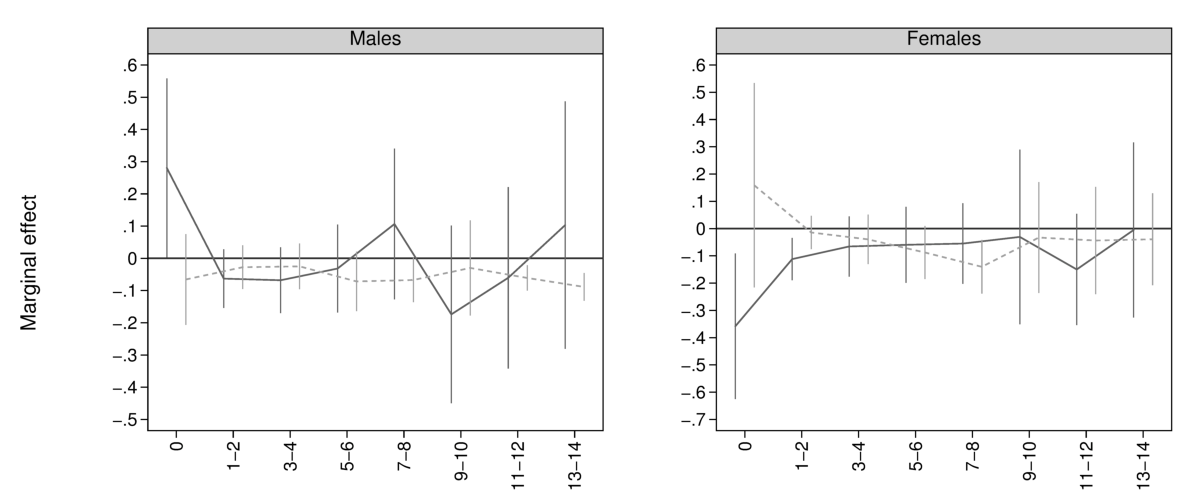
\includegraphics[width=\linewidth]{Chapter5/Figures/mi_obese_fe}
%Marginal structural models
%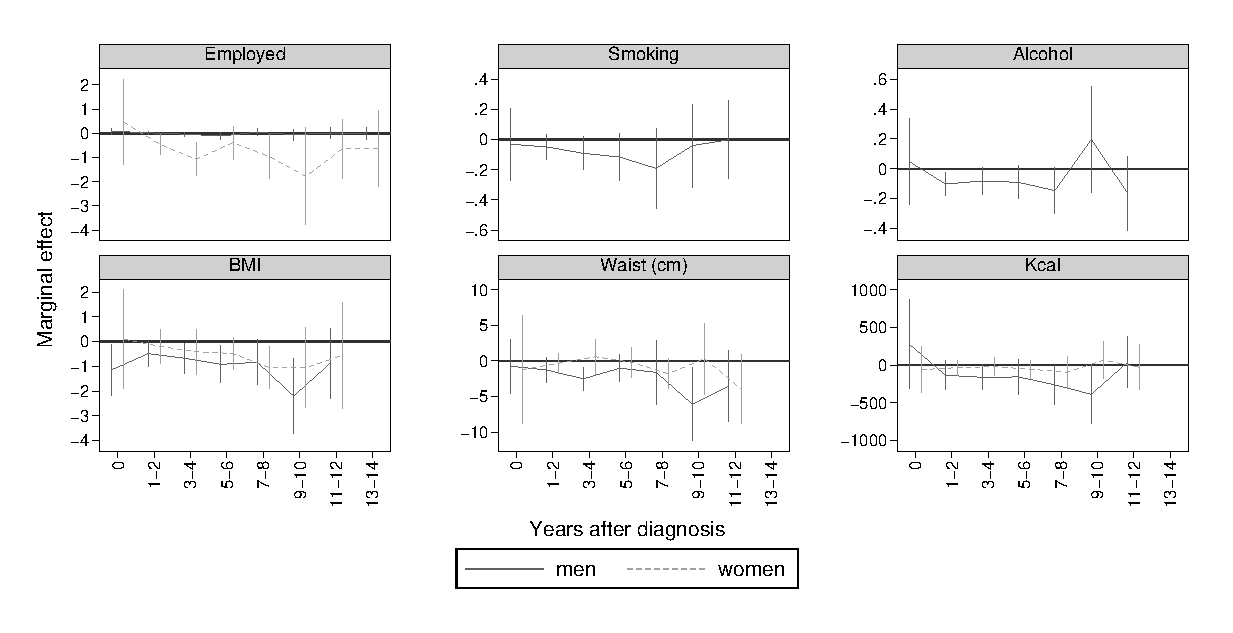
\includegraphics[width=\linewidth]{Chapter5/Figures/mi_msm_l_all}
\end{center}
\end{figure}
